\documentclass{article}

\usepackage{amsmath}
\usepackage{amsfonts}
\usepackage{ mathrsfs }
\usepackage{tikz}
\usetikzlibrary{cd}

\begin{document}
	
	
	
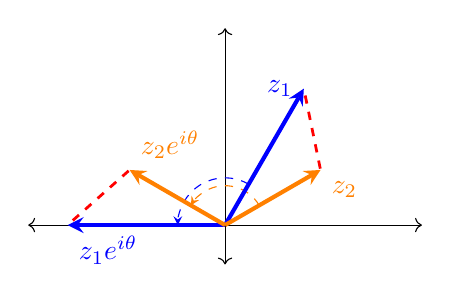
\begin{tikzpicture}

  %% Axis
  \draw[<->] (-2.5,0)--(2.5,0);%% node[above]{$\operatorname{Re}\{z\}$};
  \draw[<->] (0,-0.5)--(0,2.5);%% node[above]{$\operatorname{Im}\{z\}$};
  
   \draw[blue, -stealth, dashed](0.3, 0.5196) arc(60:180:0.6);
  \draw[orange, -stealth, dashed](0.433, 0.25) arc(30:150:0.5);
  
  %% Original vectors
  \draw[line width=1.5pt,blue,-stealth](0,0)--(1, 1.732) node[anchor=  east]{${z_1}$};
  \draw[line width=1.5pt,orange,-stealth](0,0)--(1.2124, 0.7) node[anchor= north west]{${z_2}$};
  \draw[line width=1pt,red, dashed, shorten <=2.5](1, 1.732)--(1.2124, 0.7);% node[anchor= south west]{${| z_1 - z_2| }$};
  

  
  %% Rotated vectors
  \draw[line width=1.5pt,blue,-stealth](0,0)--(-2, 0) node[anchor= north west]{${z_1 e^{i\theta}}$};
  \draw[line width=1.5pt,orange,-stealth](0,0)--(-1.2124, 0.7) node[anchor= south west]{${z_2 e^{i\theta}}$};
  \draw[line width=1pt,red, dashed, shorten <=2.5](-2, 0)--(-1.2124, 0.7);% node[anchor= south east]{${| z_1e^{i\theta} - z_2e^{i\theta}| }$};
  
\end{tikzpicture}


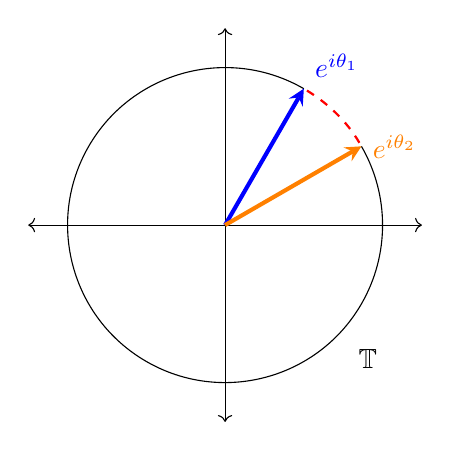
\begin{tikzpicture}

%% Axis
\draw[<->] (-2.5,0)--(2.5,0) ; %%node[right]{$\operatorname{Re}\{z\}$};
\draw[<->] (0,-2.5)--(0,2.5) ; %%node[above]{$\operatorname{Im}\{z\}$};

% Unit circle
 \draw(1, 1.732) arc(60:390:2);
 \draw[red, thick, dashed, shorten <=1.5] (1.732, 1) arc(30:60:2);
 \node[text width=0.2] at (1.7,-1.7) {$\mathbb{T}$};

%% Original vectors
\draw[line width=1.5pt,blue,-stealth](0,0)--(1, 1.732) node[anchor=  south west]{${e^{i \theta_1}}$};
\draw[line width=1.5pt,orange,-stealth](0,0)--(1.732, 1) node[anchor=  west]{${e^{i \theta_2}}$};



\end{tikzpicture}
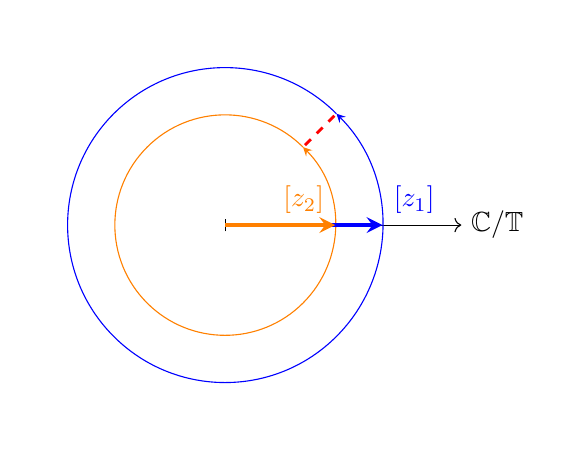
\begin{tikzpicture}

%% Fake axes to have the same margins
\draw[white, opacity=0] (-2.5,0)--(2.5,0) ; %%node[right]{$\operatorname{Re}\{z\}$};
\draw[white, opacity=0] (0,-2.5)--(0,2.5) ; %%node[above]{$\operatorname{Im}\{z\}$};

%% Axis
\draw[|->] (0,0)--(3,0) node[right]{$\mathbb{C}/\mathbb{T}$};


%%\draw[orange] (0, 0) circle (1.4);
%%\draw[blue] (0, 0) circle (2);

 \draw[orange, -stealth] (0.9899, 0.9899) arc(45:405:1.4);
 \draw[blue, -stealth] (1.4142, 1.4142) arc(45:405:2);

%% Rotated vectors
\draw[line width=1.5pt,blue,-stealth](0,0)--(2, 0) node[anchor= south west]{${[z_1]}$};
\draw[line width=1.5pt,orange,-stealth](0,0)--(1.4, 0) node[anchor= south east]{${[z_2]}$};
\draw[line width=1pt,red, dashed, shorten <=1](0.9899, 0.9899)--(1.4142, 1.4142);% node[anchor= south west]{$|[z_1] - [z_2]|$};




\end{tikzpicture}



%% Start Figure:
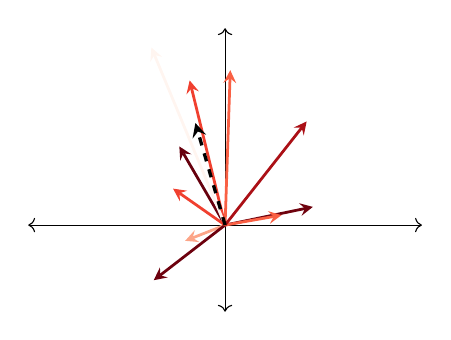
\begin{tikzpicture}
%% Axis
\draw[<->] (-2.5,0)--(2.5,0);% node[above]{$\operatorname{Re}\{z\}$};
\draw[<->] (0,-1.1)--(0,2.5);% node[above]{$\operatorname{Im}\{z\}$};
%%Vectors colored
\definecolor{color10}{RGB}{103,0,13}
\draw[color10, line width=1pt,-stealth](0,0)--(-0.581,0.999);
\definecolor{color11}{RGB}{252,165,136}
\draw[color11, line width=1pt,-stealth](0,0)--(-0.507,-0.2);
\definecolor{color12}{RGB}{109,1,14}
\draw[color12, line width=1pt,-stealth](0,0)--(-0.906,-0.7);
\definecolor{color13}{RGB}{240,64,47}
\draw[color13, line width=1pt,-stealth](0,0)--(-0.45,1.837);
\definecolor{color14}{RGB}{111,2,14}
\draw[color14, line width=1pt,-stealth](0,0)--(1.115,0.231);
\definecolor{color15}{RGB}{249,96,68}
\draw[color15, line width=1pt,-stealth](0,0)--(0.066,1.967);
\definecolor{color16}{RGB}{255,245,240}
\draw[color16, line width=1pt,-stealth](0,0)--(-0.936,2.255);
\definecolor{color17}{RGB}{249,96,68}
\draw[color17, line width=1pt,-stealth](0,0)--(0.717,0.126);
\definecolor{color18}{RGB}{171,16,22}
\draw[color18, line width=1pt,-stealth](0,0)--(1.036,1.316);
\definecolor{color19}{RGB}{240,64,47}
\draw[color19, line width=1pt,-stealth](0,0)--(-0.661,0.463);
%%Karcher mean of vectors
\draw[line width=1.2pt, dashed, -stealth](0,0)--(-0.377,1.296);
\end{tikzpicture}
%% Start Figure:
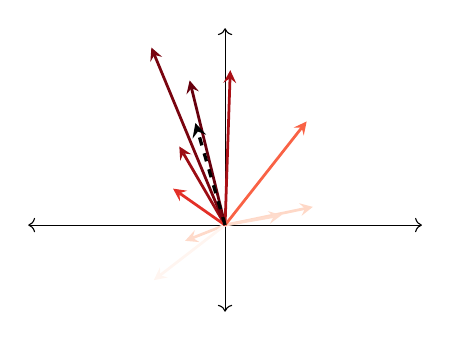
\begin{tikzpicture}
%% Axis
\draw[<->] (-2.5,0)--(2.5,0);% node[above]{$\operatorname{Re}\{z\}$};
\draw[<->] (0,-1.1)--(0,2.5);% node[above]{$\operatorname{Im}\{z\}$};
%%Vectors colored
\definecolor{color20}{RGB}{156,13,20}
\draw[color20, line width=1pt,-stealth](0,0)--(-0.581,0.999);
\definecolor{color21}{RGB}{254,218,202}
\draw[color21, line width=1pt,-stealth](0,0)--(-0.507,-0.2);
\definecolor{color22}{RGB}{255,245,240}
\draw[color22, line width=1pt,-stealth](0,0)--(-0.906,-0.7);
\definecolor{color23}{RGB}{103,0,13}
\draw[color23, line width=1pt,-stealth](0,0)--(-0.45,1.837);
\definecolor{color24}{RGB}{254,216,199}
\draw[color24, line width=1pt,-stealth](0,0)--(1.115,0.231);
\definecolor{color25}{RGB}{170,16,22}
\draw[color25, line width=1pt,-stealth](0,0)--(0.066,1.967);
\definecolor{color26}{RGB}{121,4,15}
\draw[color26, line width=1pt,-stealth](0,0)--(-0.936,2.255);
\definecolor{color27}{RGB}{254,220,205}
\draw[color27, line width=1pt,-stealth](0,0)--(0.717,0.126);
\definecolor{color28}{RGB}{249,98,69}
\draw[color28, line width=1pt,-stealth](0,0)--(1.036,1.316);
\definecolor{color29}{RGB}{227,47,39}
\draw[color29, line width=1pt,-stealth](0,0)--(-0.661,0.463);
%%Karcher mean of vectors
\draw[line width=1.2pt, dashed, -stealth](0,0)--(-0.377,1.296);
\end{tikzpicture}

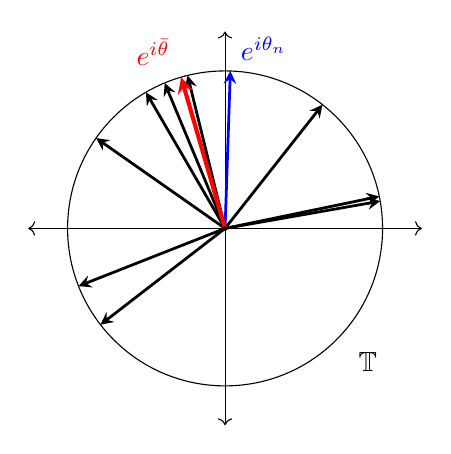
\begin{tikzpicture}

%% Axis
\draw[<->] (-2.5,0)--(2.5,0) ; %%node[right]{$\operatorname{Re}\{z\}$};
\draw[<->] (0,-2.5)--(0,2.5) ; %%node[above]{$\operatorname{Im}\{z\}$};

%% Unit circle
\draw (0, 0) circle (2);
\node[text width=0.2] at (1.7,-1.7) {$\mathbb{T}$};

%%Vectors colored
\draw[line width=1pt,-stealth](0,0)--(-1.005,1.729);
\draw[line width=1pt,-stealth](0,0)--(-1.861,-0.733);
\draw[line width=1pt,-stealth](0,0)--(-1.583,-1.223);
\draw[line width=1pt,-stealth](0,0)--(-0.476,1.942);
\draw[line width=1pt,-stealth](0,0)--(1.958,0.406);
\draw[line width=1pt,-stealth, blue](0,0)--(0.067,1.999) node[anchor= south west]{${e^{i\theta_n}}$};;
\draw[line width=1pt,-stealth](0,0)--(-0.767,1.847);
\draw[line width=1pt,-stealth](0,0)--(1.97,0.346);
\draw[line width=1pt,-stealth](0,0)--(1.237,1.571);
\draw[line width=1pt,-stealth](0,0)--(-1.638,1.147);
%%Karcher mean of vectors
\draw[line width=1.5pt, red, -stealth](0,0)--(-0.558,1.92) node[anchor= south east]{$e^{i \bar \theta}$};
\node at (0,0) [circle,fill,inner sep=0.6pt]{};
\end{tikzpicture}
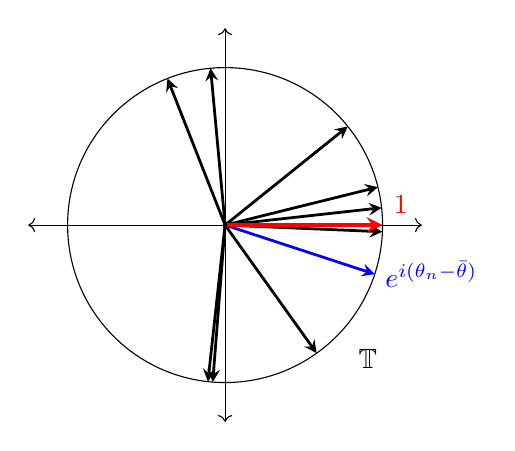
\begin{tikzpicture}

%% Axis
\draw[<->] (-2.5,0)--(2.5,0) ; %%node[right]{$\operatorname{Re}\{z\}$};
\draw[<->] (0,-2.5)--(0,2.5) ; %%node[above]{$\operatorname{Im}\{z\}$};

%% Unit circle
\draw (0, 0) circle (2);
\node[text width=0.2] at (1.7,-1.7) {$\mathbb{T}$};
%%Vectors colored
\draw[line width=1pt,-stealth](0,0)--(1.941,0.482);
\draw[line width=1pt,-stealth](0,0)--(-0.184,1.992);
\draw[line width=1pt,-stealth](0,0)--(-0.732,1.861);
\draw[line width=1pt,-stealth](0,0)--(1.998,-0.085);
\draw[line width=1pt,-stealth](0,0)--(-0.157,-1.994);
\draw[line width=1pt,-stealth, blue](0,0)--(1.901,-0.623) node[anchor= west]{${e^{i(\theta_n - \bar \theta)}}$};;
\draw[line width=1pt,-stealth](0,0)--(1.988,0.22);
\draw[line width=1pt,-stealth](0,0)--(-0.218,-1.988);
\draw[line width=1pt,-stealth](0,0)--(1.163,-1.627);
\draw[line width=1pt,-stealth](0,0)--(1.559,1.253);
%%Karcher mean of vectors
\draw[line width=1.5pt, red, -stealth](0,0)--(2,0) node[anchor= south west]{${1}$};
\node at (0,0) [circle,fill,inner sep=0.6pt]{};


\end{tikzpicture}



\begin{tikzcd}
f \arrow{r}{\text{\tiny{SRSF}}} \arrow{d}[left]{\text{action on } \mathscr{F}} & q \arrow{d}{\text{action on } \mathbb{L}^2} \\
{f \circ \gamma} \arrow{r}{\text{\tiny{SRSF}}} & {(q, \gamma)}
\end{tikzcd}


\begin{tikzcd}
	{\mathscr{F}}  \arrow[bend left=60]{r}{q_i} & 
	{\mathbb{L}^2} \arrow[bend left=60]{r}{[q_i]} \arrow[bend left=60]{l}{\tilde \mu_f } & 
	{\mathscr{A} } \arrow[bend left=60]{l}{\tilde \mu_q} 
\end{tikzcd}



\end{document}